\Chapter{Modèle plasmas froids magnétisés}
\begin{refsection}

\chaptermark{Modèle plasmas froids magnétisés}

Dans ce chapitre, nous proposons un nouveau modèle fluide pour décrire le
transport magnétisé dans les plasmas froids. Après un bref rappel de
la problématique liée à l'approche standard de modélisation des plasmas froids,
nous présentons l'élaboration d'un nouveau modèle, MAGNIS (MAGnetized Negative
Ion Source) ; nous le dérivons en expliquant les différents termes
essentiels à description du transport dans les plasmas froids puis nous détaillons le
schéma numérique original utilisé pour résoudre les équations. Enfin une
première étape de vérification du modèle est présentée à travers une étude de
convergence sur maillage.

\section{Problématique}

Comprendre l'origine et la nature du transport dans les plasmas
froids magnétisés est un enjeu majeur pour la conception, la réalisation et
l'optimisation de nombreuses applications et
procédés~\parencite{Lieberman}. Dans le domaine des plasmas froids, la plupart des modèles
fluides décrivant les phénomènes de transport magnétisés sont basés sur les
équations de Dérive-Diffusion (\S~\ref{1-deriveDiffMag}).

Cependant, à basse pression ou au delà d'une
certaine intensité de champ magnétique, la résolution numérique de ces
équations est complexe voire impossible. Ce problème ne peut alors
généralement être adressé qu'à travers le développement de modèles cinétiques
numériquement très coûteux, demandant a priori la résolution d'échelles de
l'ordre de la longueur de Debye et de la fréquence plasma.

Pour les plasmas fortement magnétisés, la description du transport transverse
par les vitesses de dérive
(cf.\S~\ref{ApproximationsEqMvt}-\ref{vitessesDerive}) fait intervenir la divergence de la dérive de
polarisation dans l'équilibre des courants~\parencite{Tamain2}. Cette dérive,
essentielle dans la dynamique du transport transverse en présence d'un fort champ magnétique, est
absente du modèle de Dérive-Duffusion qui néglige totalement l'inertie des
particules.
Les modèles de Dérive-Diffusion, en cherchant une solution stationnaire à un
problème intrinsèquement non-stationnaire, sont en fait peu adaptées pour décrire le
transport fortement magnétisé~\parencite{Fruchtman,Sternberg}.

Nous adressons la complexité de ce transport à travers l’élaboration d'un modèle
fluide sans approximation d'ordering entre les longueurs caractéristiques du
plasma magnétisé (i.e. la dimension du plasma $L$, les libres parcours moyens
$\lambda_{i,e}$ et les rayons de Larmor ioniques et électroniques $\rho_{Li,e}$). 
La prise en compte de l'inertie	dans les équations de transport nous permet de
plus de capturer la dynamique transitoire du plasma, comme certains types
d'instabilités. Ce modèle fluide dynamique peut être utilisé pour explorer
une large gamme de topologies et d'intensités de champ magnétique.

\section{Description du modèle}
Le plasma est constitué d'électrons et d'une ou plusieurs espèces d'ions, de
charge $q_\alpha$ et de masse $m_\alpha$. On considère un plasma de taille $L$,
confiné et en interaction avec des parois à travers une gaine large de quelques longueurs
de Debye. La longueur $L$ est prise suffisamment grande $L\gg\lambda_D$ pour
supposer le plasma quasineutre. Le champ magnétique $\mathbf{B}$ imposé est 
stationnaire, de sorte que le champ électrique dérive directement d'un 
potentiel électrostatique $\mathbf{E}=-\nabla \Phi$. Le transport est décrit
dans le plan perpendiculaire au champ magnétique et les conditions aux limites
parallèles, qui dérivent d'une théorie classique de gaine, sont
incluses directement dans les équations de conservation à travers des termes
sources effectifs. L'équation d'énergie tient compte des pertes
associées à l'ensemble des collisions (dont celles dues à l'ionisation des particules) et
contient un terme de puissance
absorbée avec un profil fixé. Enfin, le flux de chaleur magnétisé
est décrit par une équation dédiée.

Le modèle, construit sans approximation d'échelle (excepté sur $\lambda_D$),
permet la résolution du transport magnétisé quelque soit l'ordering entre les
libres parcours moyens $\lambda_{{i/e}}$, les rayons de Larmor ioniques et
électroniques $\rho_{L{i/Le}}$ et la taille $L$ du plasma :
\begin{equation}
\lambda_D\ll\underbrace{\rho_{L{i/Le}},\lambda_{{i/e}},L}_\text{ordering
arbitraire}
\end{equation}

\subsection{Équations de conservation}
Pour décrire l'évolution des espèces dans un plasma partiellement ionisé, basse
pression et magnétisé, l'équation de la quantité de mouvement doit tenir compte
de l'interaction avec le gaz, du terme de Laplace et de l'inertie :

\begin{equation}
\label{3-eqMouvement}
\partial_t \mathbf{u}_\alpha + \mathbf{u}_\alpha\cdot\nabla\mathbf{u}_\alpha+
\nu_\alpha\mathbf{u}_\alpha+\omega_{c\alpha}\mathbf{b}\times\mathbf{u}_\alpha=
-\frac{q_\alpha}{m_\alpha}\left(\nabla \Phi+\frac{\nabla
p_\alpha}{q_\alpha n_\alpha}\right)
\end{equation}

où $n_\alpha$ est la densité de l'espèce considérée, $\mathbf{u}_\alpha$ sa
vitesse fluide, $p_\alpha =en_\alpha T_\alpha$ la pression (dont nous ne
retenons que la contribution isotrope) et $\Phi$ le potentiel électrostatique. La fréquence
cyclotronique est notée $\omega_{c\alpha}=q_\alpha B/m_\alpha$ et $\nu_\alpha$
est une fréquence effective rendant compte des collisions :

\begin{equation}
\nu_\alpha=\nu_{\alpha}^\text{iz}+\nu_{\alpha}^{c}
\end{equation}

Le transfert de quantité de mouvement dû aux collisions contient la perte liée à
l'ionisation à travers la fréquence $\nu_{\alpha}^\text{iz}$, primordiale dans
la description des plasmas froids. $\nu_{\alpha}^{c}$ regroupe l'ensemble des
collisions élastiques, essentiellement avec le gaz, mais aussi éventuellement
entre les espèces chargées (collisions coulombiennes). En présence de plusieurs espèces, la
fréquence $\nu_{\alpha}^{c}$, résultat de toutes les interactions, s'écrit :

\begin{equation}
\nu_{\alpha}^c=n_\alpha\sum_{s\neq\alpha} \frac{m_s}{m_\alpha+m_s}
n_sk^m_{\alpha s}
\end{equation}

où $k^m_{\alpha
s}=\left<\sigma^m_{\alpha s}v_r\right>$ est un taux de transfert de quantité de
mouvement spécifique à la réaction considérée, $\sigma^m_{\alpha s}$ étant la
section efficace de l'interaction et $v_r$ la vitesse relative des particules en
collision (voir \S~\ref{Introduction}-\ref{1-Collisions}). Un grand nombre
d'interactions et de réactions chimiques peuvent éventuellement être prises en compte avec cette description.

L'évolution de chaque espèce est décrite par une équation de continuité :

\begin{equation}
\label{3-continuite}
\partial_t n_\alpha +
\nabla\cdot\left(n_\alpha\mathbf{u}_\alpha\right)=\mathcal{S}_\alpha(T_e)
\end{equation}

avec $\mathcal{S}_\alpha$ un terme source net, fortement dépendant de la
température électronique $T_e$. Dans le cas simple d'un plasma mono-espèce avec
l'ionisation comme seule réaction inélastique, ce terme se réécrit :

\begin{equation}
\mathcal S_e=\mathcal
S_i=n_e\nu_\text{iz}=n_en_gk^\text{iz}(T_e) 
\end{equation}

En considérant l'hypothèse de quasineutralité, la
somme des équations de continuité conduit à l'équation de conservation du courant :

\begin{equation}
\label{eqCourant}
\nabla\cdot(\sum_\alpha q_\alpha n_\alpha\mathbf
u_\alpha)=\nabla\cdot(\sum_iq_in_i\mathbf{u}_i-en_e\mathbf{u}_e)=0
\end{equation}

où l'indice $i$ dénote éventuellement différentes espèces d'ions, positifs ou
négatifs.
L'équation \eqref{eqCourant} couple l'ensemble des espèces en contrôlant
l'évolution du potentiel électrostatique $\Phi$.

L'équation de conservation de l'énergie est obtenue classiquement en substituant
l'équation de continuité afin d'éliminer le terme convectif puis en retranchant
l'expression de l'énergie dirigée $\mathcal{U}_e=m_eu_e^2/2$
(cf.~\eqref{1-eqEnergieInterne}) :

\begin{equation}
\label{3-eqTemperature}
\frac{3}{2}n_e\frac{\text{d}T_e}{\text{dt}}+\nabla\cdot\mathbf
q_e + \frac{5}{2}\mathcal{S}_e T_e = T_e\frac{\text{d}n_e}{\text{dt}}+ 
en_e\left(\mathcal{P}_\text{ext}+\Pi_e\right)+(2n_e\nu_e+\mathcal{S}_e)\mathcal{U}_e
\end{equation}

où $T_e$ est la température électronique exprimée en unité d'énergie,
$\text{d/dt}=\partial_t+u_e\cdot\nabla$ représente la dérivée totale et
$\mathcal{S}_e$ est le terme source d'électrons lié à l'ionisation. 
Le chauffage ohmique, conséquence du travail du champ électrique transformé en
chaleur par l'intermédiaire des collisions, n'apparaît pas explicitement en
fonction du champ électrique mais est inclus dans le terme
$(2n_e\nu_e+\mathcal{S}_e)\mathcal{U}_e$. L'ajout d'énergie dans le plasma, par
exemple avec un chauffage RF, est modélisé par un terme
de puissance absorbée $\mathcal{P}_\text{ext}$, que nous imposons avec un
certain profil. Enfin, le terme de perte d'énergie due aux collisions $\Pi_e$,
dépendant de la température électronique, se décompose en une perte lié à
l'ionisation et un terme de transfert vers les autres espèces :

\begin{equation}
en_e\Pi_e(T_e)
=-en_e\left(\sum_{s}E_sn_sk_{es}(T_e)+\sum_{s'}\frac{3m_e}{m_{s'}}n_s'k^m_{es'}(T_e)T_e\right)
\equiv-en_en_gk^\varepsilon_e(T_e)
\end{equation}


avec $k_e^\varepsilon$ un taux effectif de transfert d'énergie (sommé sur 
l'ensemble des processus de collision, y compris les auto-collisions).
La fermeture du modèle se fait sur le flux de chaleur $\mathbf{q}_e$, tel qu'exprimé par V.E. Golant
dans~\parencite{Golant} :

\begin{equation}
\label{3-eqFluxChaleur}
\partial_t \mathbf{q}_e + \nu_e\mathbf{q}_e+\omega_e\mathbf{q}_e\times\mathbf{b} =
-\frac{5}{2}\frac{n_eT_e}{m_e}\nabla T_e
\end{equation}

Le gradient de température, moteur du flux de chaleur, est multiplié par le
facteur $5n_eT_e/2m_e$, approximation classique pour refermer le
système~\parencite{bittencourt}.
Dans les sources magnétisées,
où la longueur de gradient thermique est de l'ordre de la largeur
du filtre magnétique, le flux de chaleur est magnétisé de la même façon que le
flux de matière et influence fortement le transport transverse. Il doit donc
nécessairement être pris en compte et décrit avec le minimum d'approximations.

\subsection{Conditions aux limites}
Le modèle quasineutre est complété par la
définition de conditions aux limites portant sur les flux et intégrant le
maximum de considérations physiques en fonction de la nature conductrice ou
diélectrique de la paroi.
Un modèle classique de gaine non-collisionnelle positive est utilisé. Pour
l'équation de continuité \eqref{3-continuite}, un flux net de
particules est imposé à la surface :

\begin{equation}
	\Gamma_\alpha=n_\alpha\mathbf u_\alpha\cdot \mathbf n=n_\alpha W_\alpha
\end{equation} 

avec $\mathbf{n}$ le vecteur normal à la paroi et $W_\alpha$ une vitesse de
perte effective de l'espèce en entrée de gaine. Les flux d'ions
positifs\footnote{Le comportement des ions négatifs est à rapprocher de celui
des électrons. Enfermés dans le puit de potentiel, les ions négatifs
suivent eux aussi une distribution de Boltzmann. Leur prise en compte complique
cependant l'écriture des conditions aux bords du
plasma et, dans l'objectif de garder les équations claires, nous ne présentons
dans ce manuscrit que le cas des ions positifs.} sont définis par :

\begin{equation}
\label{3-fluxIonique}
\Gamma_i=n_iW_i=n_i\max\left(c_{si},\mathbf{u_i}\cdot\mathbf{n}\right)
\end{equation}

où $c_{si}=(T_e/m_i)^{\text{\textonehalf}}$ est la vitesse de Bohm
spécifique à l'espèce $i$.
Chaque espèce ionique atteint donc au minimum sa propre vitesse de Bohm, mais
peut éventuellement être perdue avec une vitesse
supersonique\footnote{Souvent, on impose l'égalité stricte $W_i=c_{si}$ au
niveau de la gaine car la transition subsonique-supersonique est interdite dans
le plasma quand celui-ci est considéré stationnaire ou isotherme. Si ces
hypothèses ne sont pas retenues, rien n'empêche a priori à la vitesse ionique de
dépasser la vitesse de Bohm. C'est ce que nous avons constaté lors du
développement du modèle, où dans certaines situations, fixer artificiellement
$W_i$ à $c_{si}$ peut faire apparaître une accumulation de densité à la la
frontière plasma-gaine.

Ainsi, nous n'imposons qu'un minimum à la vitesse ionique, tel que défini par
le critère de Bohm et nous laissons au modèle quasineutre le soin de résoudre la
vitesse à l'intérieur du plasma.}. 

Le flux d'électrons est obtenu en considérant une fonction de distribution
maxwellienne, que l'on intègre sur le demi-espace des vitesses dirigées vers la
paroi, polarisée à $\Phi_w$, avec $v_{Te}=(T_e/m_e)^{\text{\textonehalf}}$ la
vitesse électronique thermique :

\begin{equation}
\Gamma_e=n_eW_e=n_e\frac{1}{\sqrt{2\pi}}v_{Te}=n_e\sqrt{\frac{T_e}{2\pi
m_e}}\exp(-e(\Phi-\Phi_w)/T_e)
\end{equation}

La somme des flux
ioniques et du flux électronique donne une condition limite pour l'équation de
conservation de la charge \eqref{eqCourant} en fonction de la polarisation de la paroi
:

\begin{equation}
\label{3-sheathcurrent}
\mathbf{j}\cdot\mathbf{n}=\sum_i{q_in_iW_i}
-en_e\sqrt{\frac{T_e}{2\pi
m_e}}\exp(-e(\Phi-\Phi_w)/T_e)
\end{equation}

Dans
le cas d'un plasma n'étant composé que d'une seule espèce d'ion, 
la condition \ref{3-sheathcurrent} se factorise alors en :

\begin{equation}
\mathbf{j}\cdot\mathbf{n}=en_ec_s(1-\exp(\Lambda-e(\Phi-\Phi_w)/T_e))
\end{equation}

le potentiel flottant normalisé $\Lambda=({m_i}/{2\pi
m_e})^{\text{\textonehalf}}$ est la valeur d'équilibre autour de laquelle
le potentiel plasma s'ajuste pour s'accommoder à la paroi.
Si la paroi est isolante, la surface se polarise
pour assurer la nullité du courant sortant :

\begin{equation}\begin{split}
\mathbf j\cdot\mathbf{n}=0\Leftrightarrow
\Phi_w=\Phi-\frac{T_e}{e}\ln\left(\sqrt{\frac{2\pi
m_e}{T_e}}\frac{1}{en_e}\sum_iq_in_iW_i\right)
\end{split}\end{equation}

Pour les conditions aux limites de l'équation sur la température
électronique~\eqref{3-eqTemperature}, on obtient l'énergie perdue par les
électrons en entrée de gaine en additionnant l'énergie moyenne perdue à la paroi (intégrée sur une distribution semi-maxwellienne) et l'énergie transférée aux ions dans la chute de potentiel :

\begin{equation}
	\varepsilon_w=2T_e+e(\Phi-\Phi_w)
\end{equation}
 
 On peut alors relier cette perte totale aux flux sortants de l'équation
 d'énergie \eqrefp{3-eqTemperature}, i.e. au flux d'énergie porté
 par les particules et au flux de chaleur :
 
\begin{equation}
\Gamma_\varepsilon=\frac{5}{2}{\Gamma}_eT_e+\mathbf{q}_e\cdot\mathbf{n}=
\Gamma_e\left(2T_e+e(\Phi-\Phi_w)\right)
\end{equation}

En regroupant les termes portant sur le flux d'électron, on peut exprimer la
condition limite pour le flux de chaleur :

\begin{equation}
\mathbf{q}_e\cdot\mathbf{n}=\Gamma_e\left(e(\Phi-\Phi_w)-\frac{1}{2}T_e\right)
\end{equation}

Ces conditions aux limites, dérivées de la théorie des gaines
non-collisionnelles classiques positives\footnote{En cas de
phénomène d'inversion de gaine ($\Phi$ devient inférieur à $\Phi_w$), nous
traitons le problème en réduisant la vitesse ionique du facteur de Boltzmann :
$$W_i=W_i\left(1-\exp\left(-\frac{\Phi-\Phi_w}{T_e}\right)\right)$$
Dans une situation typique où $\Phi>\Phi_w$, ce facteur est dérisoire et les
ions ont chacun leur vitesse de Bohm. Quand $\Phi\approx\Phi_w$, le facteur de
Boltzmann réduit la vitesses des ions qui ne sont plus accélérés dans la chute
de potentiel. On prévient de même la vitesse électronique de devenir trop élevée
en limitant le facteur à une valeur maximale.}, sont justifiées dans des
plasmas non-magnétisés et à l'extrémité de lignes de champ interceptant la paroi dans les plasmas magnétisés. Bien que ce choix soit discutable, nous les appliquons aussi dans la direction perpendiculaire au champ magnétique.



\subsection{Réduction 2D du modèle}

Le système d'équations Eqs.(\ref{3-continuite}~-~\ref{3-eqTemperature}) décrit le
transport magnétisé dans un plasma froid en suivant l'évolution des densités de
particules $n_\alpha$, du potentiel électrostatique $\Phi$ et de la
température électronique $T_e$ dans un espace à trois dimensions. 

Le champ magnétique n'affecte que très peu les particules dans la direction
parallèle aux lignes de champ : le plasma est stationnaire, et les électrons,
confinés par le potentiel de gaine, sont en équilibre de Boltzmann le long des
lignes.
Le problème du transport magnétisé se réduit alors essentiellement au problème du transport
dans le plan perpendiculaire à $\mathbf B$, qui est le plan des dérives et des
forts gradients.

La dissociation des mouvements parallèle et perpendiculaire s'effectue
en réécrivant les équations dans un repère axé sur le champ magnétique
(O,$\mathbf x$,$\mathbf y$,$\mathbf b$). On peut ensuite intégrer chacun des
termes le long de la direction parallèle suivant l'opération :

\begin{equation}
\text{Moyennes le long des lignes :\qquad}
\bar{X}=\frac{1}{L_\para}\int_{-L_\para/2}^{L_\para/2}X \text{d}l
\end{equation}

où $L_\para$ est la taille du plasma dans la direction du champ magnétique et
$\text{d}l$ la variation infinitésimale d'une ligne de champ.
Les divergences parallèles font intervenir les conditions aux limites au bout
des lignes de champ, qui apparaissent alors comme des termes nets de
perte $\mathcal L_\para$ dans les équations de conservation :

\begin{align}
\label{3-vitessesBord}
\begin{split}
\mathcal{L}&_{i_\para}=\frac{1}{L_\para}\int_{-L_\para/2}^{L_\para/2}\nabla_\para\left(n_iu_{i_\para}\right)dl=\frac{2a}{L_\para}n_iW_{i_\para}\\
\mathcal{L}&_{e_\para}=\frac{1}{L_\para}\int_{-L_\para/2}^{L_\para/2}\nabla_\para\left(n_eu_{e_\para}\right)dl=\frac{2}{L_\para}n_e\sqrt{\frac{T_e}{2\pi
m_e}}\exp(-e(\Phi-\Phi_{w_\para})/T_e)\\
\mathcal{L}&_{j_\para}=\frac{1}{L_\para}\int_{-L_\para/2}^{L_\para/2}\nabla_\para\left(j_\para\right)dl=\sum_i\mathcal{L}_{i_\para}-\mathcal{L}_{e_\para}\\
\mathcal{L}&_{\varepsilon_\para}=\frac{1}{L_\para}
\int_{-L_\para/2}^{L_\para/2}\nabla_\para
\left(\frac{5}{2}n_eT_eu_{e_\para}+q_{e_\para}\right)dl
=\frac{2}{L_\para}n_eW_{e_\para}(2T_e+\Phi-\Phi_{w_\para})
\end{split}
\end{align}

Pour les électrons, $\mathcal{L}_{e_\para}$ implique le potentiel de la
paroi au bout des lignes de champ $\Phi_{w_\para}$. Pour les pertes ioniques, un
facteur $a$ représente approximativement le ratio entre la densité de particules à l'entrée
de la gaine et la densité moyenne calculée le long des lignes de champ
(typiquement $a\approx\,$0.7-0.9).

En considérant l'hypothèse flûte, qui
consiste à supposer le transport rapide des fluctuations dans la direction
parallèle, l'intégration du système le long des lignes de champ magnétique
laisse les autres termes des
Eqs.(\ref{3-continuite}~-~\ref{3-eqTemperature}) quasiment inchangés.
Le système d'équation peut alors se réécrire en fonction des variables moyennées
($\bar{n}_\alpha$, $\bar{\mathbf u}_\alpha$, $\bar{T}_e$, \ldots) :

\begin{align}
\label{3-equations2D1}
\partial_t \bar{n}_\alpha& +
\nabla_\perp\cdot\left(\bar{n}_\alpha\bar{\mathbf{u}}_{\alpha_\perp}\right)=\bar{\mathcal{S}}_\alpha
- \mathcal{L}_{\alpha_\para}\\[0.5cm]
\nabla_\perp\cdot&(\sum_ie\bar{n}_i\bar{\mathbf{u}}_{i_\perp}
-e\bar{n}_e\bar{\mathbf{u}}_{e_\perp})= - \mathcal{L}_{j_\para}\\[0.5cm]
\begin{split}\frac{3}{2}\bar{n}_e&\frac{\text{d}\bar{T}_e}{\text{dt}} +
(\frac{5}{2}\bar{\mathcal{S}}_e
-\frac{\text{d}\bar{n}_e}{\text{dt}})\bar{T}_e+\nabla_\perp\cdot(\bar{\mathbf{q}}_{e_\perp})\\
&=e\bar{n}_e(\bar{\mathcal{P}}_\text{ext}-\bar{Q_e})-\mathcal{L}_{\varepsilon_\para}
+(2\bar{n}_e\bar{\nu}_e+\bar{\mathcal{S}}_e)\bar{\mathcal{U}}_e
\label{3-equations2D2}
\end{split}
\end{align}

Dans la suite, nous laissons de côté la notation de moyenne, l'indice
perpendiculaire et nous omettons volontairement l'indice $\alpha$ pour les
quantités se référant indifféremment aux ions ou aux électrons.

\section{Solution numérique}

Les équations Eqs.(\ref{3-equations2D1}~-~\ref{3-equations2D2}) sont résolues
semi-implicitement dans le temps avec une prédiction-correction des flux de
particules et de chaleur pour garantir la conservation du courant et de
l'énergie. Les variables macroscopiques sont avancées temporellement, par
petits pas de temps $\Delta t=t^{k+1}-t^k$, en suivant l'algorithme suivant :

\begin{enumerate}
  \item Calcul de toutes les fréquences $\nu^{k+1}$ pour
  chaque interaction à prendre en compte, des termes sources de particules
  $\mathcal{S}^{k+1}$ et des vitesses aux bords du domaine $W_{\para}^{k+1}$ et
  $W_{\perp}^{k+1}$
  \item Prédiction des vitesses fluides ${\overset{\sim}{\mathbf u}}^{\;k+1}$ à
  l'aide de l'équation de la quantité de mouvement \eqref{3-eqMouvement} en
  utilisant $\mathbf E^{k}$.
  \item Résolution du champ électrique $\mathbf E^{k+1}$ et du potentiel
  électrostatique $\Phi^{k+1}$ à travers la conservation du courant, en
  s'appuyant sur la réponse des vitesses fluides au changement $\Delta \mathbf
  E=\mathbf E^{k+1}-\mathbf E^{k}$.
  \item Correction des vitesses fluides $\mathbf u^{k+1}$ pour le nouveau
  $\mathbf E^{k+1}$.
  \item Résolution des équations de continuité ioniques \eqref{3-continuite} avec les
  vitesses corrigées $\mathbf u^{k+1}$.
  \item Calcul de la densité électronique en utilisant l'hypothèse de
  quasineutralité.
  \item Prédiction du flux de chaleur ${\overset{\sim}{\mathbf q}}_e^{\;k+1}$
  (de la même manière que pour le flux de particules) d'après
  \eqref{3-eqFluxChaleur}.
  \item Résolution de la température électronique $T_e^{k+1}$ à partir de
  l'équation de conservation de l'énergie \eqref{3-eqTemperature}, en incluant la réponse du flux de
  chaleur au changement $\Delta T_e=T_e^{k+1}-T_e^{k}$.
  \item Correction du flux de chaleur $\mathbf
  q_e^{k+1}$ pour tenir compte du changement de la température $\Delta T_e$.
\end{enumerate}

\begin{figure}[!htbp]
\centering
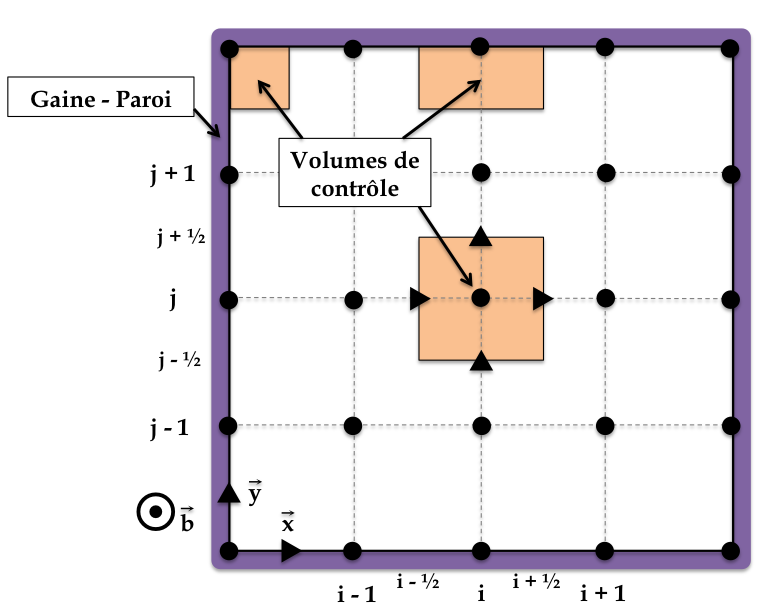
\includegraphics[width=0.5\textwidth]{figures/3-magnisGrid.png}
{\caption{Schéma du domaine de simulation, avec à sa frontière une gaine
non-collisionnelle positive.
Les quantités scalaires $n$, $\Phi$ et $T_e$ sont définies aux noeuds et sur les
bords du maillage. Les composantes $x$ et $y$ des champs vectoriels sont
situées entre les n\oe uds, sur les arêtes des volumes de contrôle,
respectivement au niveau des flèches horizontales et verticales.}
\label{3-maillage}}
\end{figure}

Le domaine de simulation est schématiquement représenté sur la figure~\ref{3-maillage}.
C'est le plan perpendiculaire à $\mathbf{b}$, rectangulaire et maillé uniformément suivant
les directions $\mathbf{x}$ et $\mathbf{y}$. Les quantités
scalaires sont définies aux noeuds du maillage ainsi que sur les bords du
domaine, et se repèrent par les indices $(i,j)$. Les quantités vectorielles
sont définies à mi-chemin entre les noeuds, aux indices $(i+1/2,j)$ pour leur
composante selon $x$ et $(i,j+1/2)$ pour leur composante selon $y$.
Les opérateurs
de divergence, quant à eux, sont discrétisés autour des volumes de contrôles en
suivant une méthode de Volumes Finis~\parencite{toro}, les volumes de
contrôle étant définis autour des n\oe uds du maillages. 

Les parois perpendiculaires et parallèles peuvent être choisies conductrices ou
isolantes, impliquant le jeu de conditions aux limites adapté sur les flux
aux bords du domaine. Le domaine peut aussi être choisi périodique dans l'une
des directions pour représenter certaines géométries, et éventuellement
de longueur infinie dans la direction parallèle.
 
Pour résoudre les systèmes linéaires du modèle, nous utilisons un solveur
9-points basé sur la procédure
MSI (Modified Strongly Implicit) décrite par Schneider
dans~\parencite{Schneider}. Sa principale caractéristique est de tenir
compte du caractère intrinsèquement lié des équations fluides afin de diminuer
le nombre d'itérations nécessaires pour trouver la solution du problème. Autorisant des
conditions aux limites périodiques, le solveur est de plus construit pour
utiliser une approche multigrille~\parencite{Fedorenko} rendant la convergence
particulièrement rapide sur un maillage 2D.

\subsection{Fréquences, termes sources et conditions aux limites}
Avant de résoudre à proprement dit les équations du modèle, à chaque
itération et pour chaque interaction, MAGNIS lit les taux $k_\text{iz}$,
$k^m_{\alpha s}$ et $k^\varepsilon_{e}$ dans des tables en fonction
de l'énergie des particules. 
Les taux contenus dans ces tables
sont issus de LXCAT~\parencite{LXCAT} : pour les électrons, ils
sont obtenus en intégrant les sections efficaces sur une distribution
maxwellienne ou en résolvant directement l'équation de
Boltzmann~\parencite{Bolsig}. Pour les ions, nous supposons la limite
basse-énergie et nous choisissons des taux constants, calculés lors
d'expériences dites de "swarm"~\parencite{Ellis}.
Ces valeurs sont illustrées pour les électrons sur la
figure~\ref{3-tauxcollision}.

\begin{figure}[!htbp]
    \centering
    \subfigure[]{\label{3-coeffColl1}
    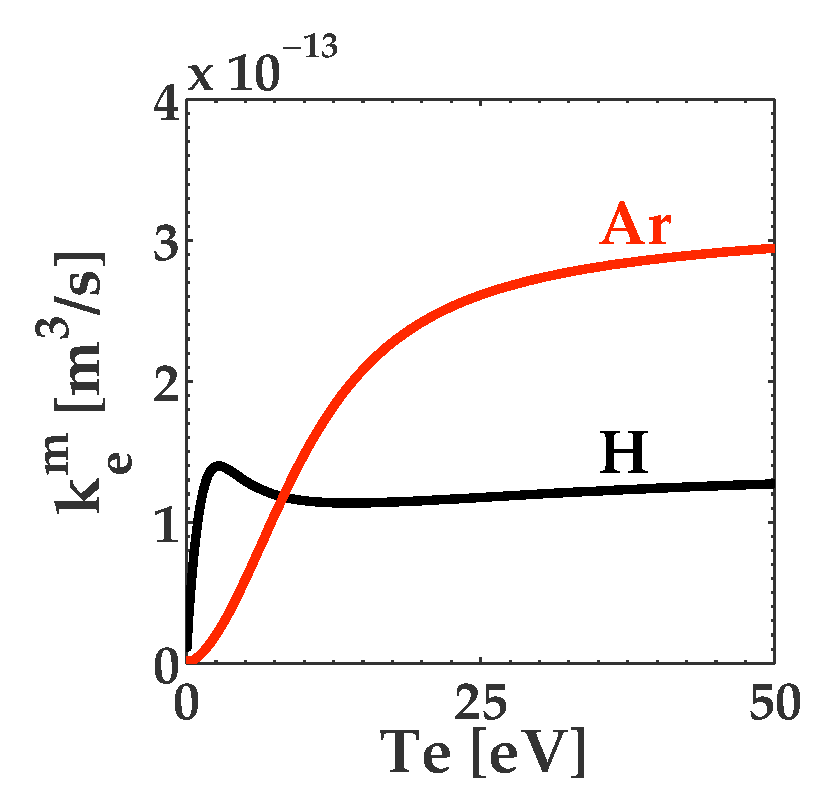
\includegraphics[width=0.3\textwidth]{figures/3-coeffColl1.eps}}
    \subfigure[]{\label{3-coeffColl2}
    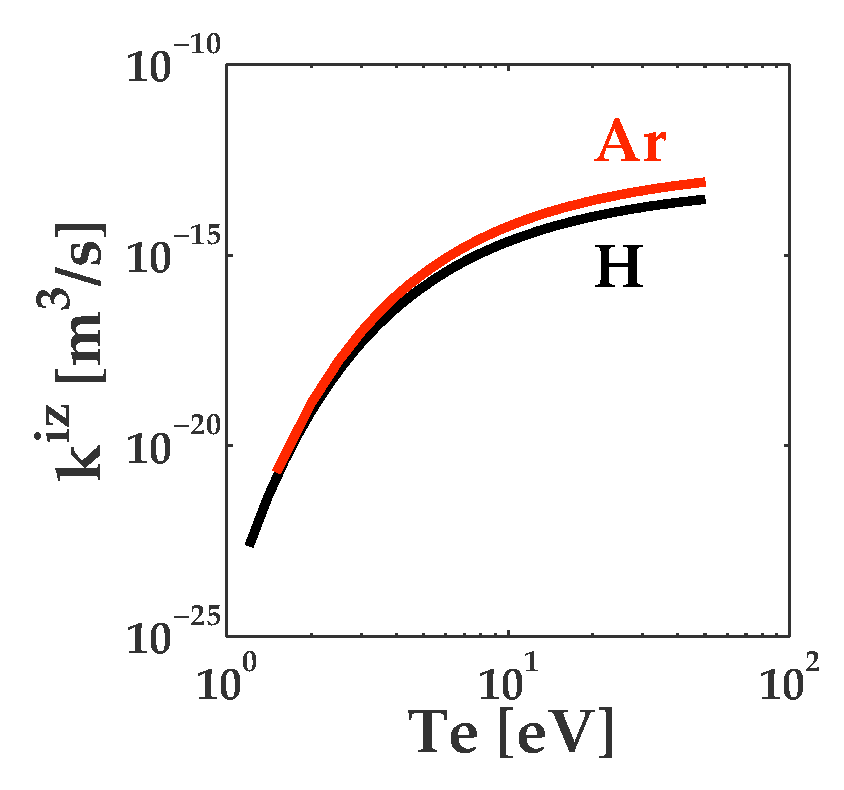
\includegraphics[width=0.3\textwidth]{figures/3-coeffColl2.eps}}
    \subfigure[]{\label{3-coeffColl3}
    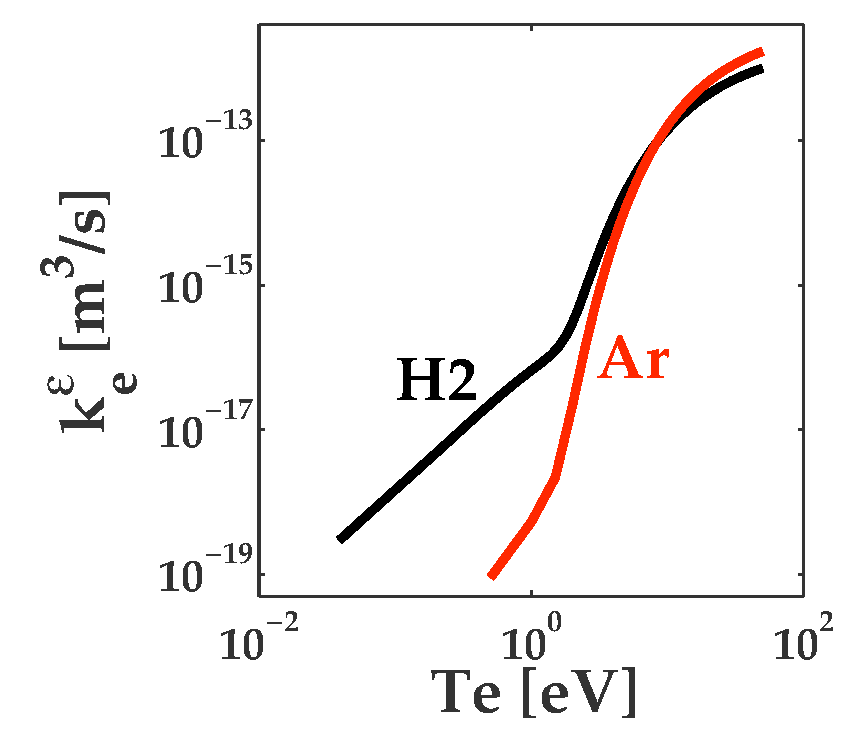
\includegraphics[width=0.3\textwidth]{figures/3-coeffColl3.eps}}
    \caption{Valeur en fonction de la température électronique des taux
    ~\subref{3-coeffColl1} de collision électrons-neutres,
    ~\subref{3-coeffColl2} d'ionisation et~\subref{3-coeffColl3} de perte
    d'énergie dans des gaz de dihydrogène et d'argon~\parencite{siglo}.}
    \label{3-tauxcollision}
\end{figure}

Le terme source de particules est calculé en fonction de la fréquence
d'ionisation et pris en compte implicitement :

\begin{equation}
\mathcal{S}_{\alpha}=n_\alpha^{k+1} \nu_\alpha^\text{iz}=n_\alpha^{k+1} n_g
k_{\alpha}^\text{iz}(T_e)
\end{equation}

Le terme de perte d'énergie par électron est lui aussi fortement dépendant de la
température électronique. Afin de
résoudre l'évolution de la température, ce terme est décomposé par une itération
de Newton\footnote{Cette technique peut être utilisée en toute généralité pour
renforcer la stabilité numérique en présence de pertes lorsque celles-ci
dépendent fortement de la quantité perdue 
$\frac{d\mathcal L}{d\mathcal Q}<0$.
La perte est alors décomposée suivant une itération de Newton pour
réaliser une prédiction implicite et atténuer son influence :
\begin{equation*}
\mathcal L^{k+1}=\mathcal L^{k}+\frac{d\mathcal L^{k}}{d\mathcal Q}(\mathcal
Q^{k+1}-\mathcal Q^k) \end{equation*}
Originalement mise en \oe uvre dans~\parencite{HagelaarImpl}, nous utilisons
cette technique pour quelques termes du modèle.} pour faire une prédiction implicite :

\begin{equation}
en_e\Pi_e(T_e^{k+1})=en_e\left(\Pi_e(T_e^{k})+\frac{\partial \Pi_e}{\partial
T_e}\left(T_e^{k+1}-T_e^{k}\right)\right)= en_en_g\left(k_e^\varepsilon+
\frac{\partial k_e^\varepsilon}{\partial T_e}(T_e^{k+1}-T_e^{k})\right)
\end{equation}


Enfin, les vitesses des particules au niveau des parois sont calculées en
fonction de leur nature isolante, conductrice ou polarisée (les expressions
sont données dans \ref{3-vitessesBord}) puis prisent en compte implicitement
dans les équations de continuité.

\subsection{Discrétisation des vitesses et interpolation}
L'un des points clés du modèle tient à la méthode de résolution de l'équation de
la quantité de mouvement et de la conservation du courant. Écrivons
\eqref{3-eqMouvement} comme une équation algébrique d'inconnue $\mathbf u$, reliant la fréquence caractéristique du transport
$\omega\sim\partial_t$, une fréquence de collision effective $\nu_m$ et la
fréquence cyclotronique $\omega_c$ avec un champ
accélérateur $\mathbf F$ incluant le terme inertiel d'advection :

\begin{equation}
\label{3-eqMvt}
\alpha_\omega\partial_t \mathbf{u} + 
\nu_m\mathbf{u}+\omega_{c}\mathbf{b}\times\mathbf{u}=
\mathbf F
\end{equation}

avec 
\begin{equation}\mathbf F=\frac{q}{m}E-\frac{\nabla
n T}{m
n}-\alpha_u\mathbf{u}\cdot\nabla\mathbf{u}
\end{equation}

Les facteurs $\alpha_\omega$ et $\alpha_u$ sont des paramètres numériques qui
permettent de modifier l'influence des termes d'inertie, ou éventuellement de
les négliger ($\alpha_{\omega,u}$=0). Discrétisons temporellement
\eqref{3-eqMvt} en prenant la vitesse implicitement dans les termes
magnétique et collisionnel\footnote{Une récente modification permet de choisir
une résolution implicite du terme
d'inertie $\mathbf{u}\cdot\nabla\mathbf{u}$, rendant le code MAGNIS
full-implicit. Cependant cela n'apporte pas d'améliorations significatives sur
les résultats, et pour des raisons de lisibilité, nous le laisserons inclus dans
la force $\mathbf F$.} :

\begin{equation}
\label{3-eqMvtDiscretT}
\delta\left(\mathbf{u}^{k+1}-\mathbf{u}^{k}\right) + 
\nu_m\mathbf{u}^{k+1}+\omega_{c}\mathbf{b}\times\mathbf{u}^{k+1}=
\mathbf F
\end{equation}

où $\delta=\alpha_\omega/\Delta t$. En combinant \ref{3-eqMvtDiscretT} et
l'expression de son produit vectoriel par $\mathbf b$, on peut éliminer le
terme de Laplace. La vitesse s'exprime alors comme une somme pondérée du
transport perpendiculaire et du transport croisé :

\begin{equation}
\label{3-eqMvtPonderee1}
\mathbf{u}^{k+1}=\text{A}_u\left(\mathbf F + \delta\mathbf{u}^{k}\right)+
\text{B}_u\mathbf b\times\left(\mathbf F + \delta\mathbf{u}^{k}\right)
\end{equation}
avec 
\begin{equation}
\label{3-coefficientsVitesses}
\text{A}_u=\frac{\nu_m+\delta}{(\nu_m+\delta)^2+\omega_c^2}\;\;\;\;\text{et}\;\;\;\text{B}_u=-\frac{\omega_c}{(\nu_m+\delta)^2+\omega_c^2}
\end{equation}

L'interpolation spatiale nécessaire à l'évaluation du
deuxième terme de \eqref{3-eqMvtPonderee1} mène
inexorablement à l'introduction d'une erreur dans l'évolution de la vitesse. Au
bout d'un grand nombre de $\Delta t$, cette erreur peut se propager à
l'ensemble des points et s'accumuler, entraînant de sérieux problèmes de convergence à petit
pas de temps. Pour remédier à ce problème, nous limitons l'erreur
d'interpolation en suivant à la fois la vitesse $\mathbf u$ et la vitesse
croisée $\mathbf u_\times=\mathbf b\times\mathbf u$ sur tous les points du
maillage :

\begin{equation}
\label{3-eqMvtPonderee12}
\mathbf{u}^{k+1}=\text{A}_u\left(\mathbf F + \delta\mathbf{u}^{k}\right)+
\text{B}_u\left(\mathbf b\times\mathbf F +
\delta\left((1-\beta)\mathbf{u}_\times^{k}+\beta\mathbf
b\times\mathbf{u}^{k}\right)\right)
\end{equation}
\begin{equation}
\label{3-eqMvtPonderee2}
\mathbf{u}_\times^{k+1}=-\text{B}_u\left(\mathbf F +
\delta\mathbf{u}^{k}\right)+ \text{A}_u\left(\mathbf
b\times\mathbf F +
\delta\left((1-\beta)\mathbf{u}_\times^{k}+\beta\mathbf
b\times\mathbf{u}^{k}\right)\right)
\end{equation}

\begin{figure}[!htbp]
\centering
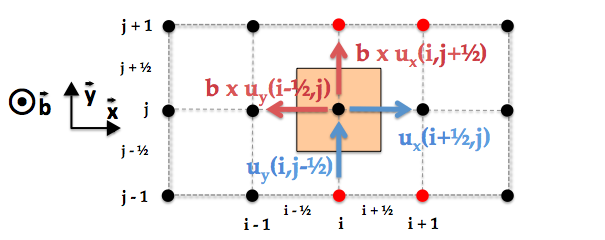
\includegraphics[width=0.8\textwidth]{figures/3-magnisVectCross.png}
{\captionsetup{justification=raggedright,
singlelinecheck=false}\label{3-magnisVectCross}\caption{Schéma de définition
des vitesses fluides et des vitesses croisées : les composantes vectorielles en
$x$ des vitesses, $\mathbf u_{|_x}$ et $\mathbf u_{\times|_x}=(\mathbf
b\times\mathbf u_y)_{|_x}$, sont définies aux mêmes points. \\ Les points de
maillage en rouge sont impliqués dans l'interpolation classique de la composante $x$ des gradients à l'origine des flux de dérive.
 Par exemple pour obtenir le champ $\mathbf{E}_\times$ en~($i$+1/2 ,$\,j$)~:
 $$\widetilde{E}_{\times}^{(i+1/2,j)}={\widetilde{\nabla_y
 \Phi}}^{(i+1/2,j)}=\frac{1}{4\Delta
 y}(\Phi^{(i+1,j+1)}-\Phi^{(i-1,j+1)}+\Phi^{(i,j+1)}-\Phi^{(i,j-1)})$$ }}
\end{figure}

Le coefficient $\beta$ est un paramètre donnant un contrôle sur
l'utilisation de ce maillage secondaire. Quand $\beta\,$= 0, aucune
interpolation n'est nécessaire, mais $\mathbf{u}$ et $\mathbf{u}_\times$
tendent à se désynchroniser et le schéma numérique diverge vite. Il faut en
fait un minimum d'interpolation $\beta\,$> 0 pour garder les vitesses
consistantes entre elles (tout en gardant en tête que trop d'interpolation
$\beta\rightarrow\,$1 mène à une explosion de l'erreur à petit pas de temps). Un
calcul analytique pour estimer l'erreur d'interpolation montre qu'un choix approprié pour le paramètre $\beta$
est :

\begin{equation}
\label{3-eqMvtPonderee3}
\beta=\left(\frac{\nu^2+\omega_c^2}{(\delta+\nu)^2+\omega_c^2}\right)^{1/2}
\end{equation}

avec cette valeur, le schéma numérique converge proprement pour n'importe quel
ordering entre $\nu$, $\omega_c$ et $\delta$.


\subsection{Conservation du courant et correction des vitesses}
\subsubsection{Prédiction et correction}

Les expressions obtenues pour les vitesses
fluides (\eqref{3-eqMvtPonderee12} et \eqref{3-eqMvtPonderee2}) font intervenir
le champ électrique à travers le terme $\mathbf F$.
L'évaluation de ce terme avec un champ électrique pris au temps $k$+1 peut alors
s'écrire en fonction du changement de potentiel :

\begin{equation}
\label{3-eqCorrection}
\mathbf F(\mathbf E^{k+1}) = \mathbf F(\mathbf E^{k})-\frac{q}{m}\nabla
(\Phi^{k+1}-\Phi^{k})
\end{equation}

La propriété \eqref{3-eqCorrection} est mise à profit afin de construire un
schéma de prédiction-correction pour les vitesses fluides. Celles-ci sont
calculées explicitement dans une première étape à partir des
équations~\eqref{3-eqMvtPonderee12} et \eqref{3-eqMvtPonderee2} avec 
l'ancien champ électrique :

\begin{equation}
\tilde{\mathbf u}^{k+1}(\mathbf{E}^k)=\text{A}_u\mathbf F(\mathbf E^{k}) +
\text{B}_u\mathbf b\times\mathbf F(\mathbf E^{k}) + \text{\ldots}
\end{equation}

puis corrigées par le changement de champ électrique
$\nabla\varphi=\nabla(\Phi^{k+1}-\Phi^k)$ :

\begin{equation}
\label{3-eqCorrectionVitesse}
\mathbf u^{k+1}(\mathbf{E}^{k+1}) = \tilde{\mathbf
u}^{k+1}(\mathbf{E}^k)-\frac{q}{m}\text{A}_u\nabla
\varphi-\frac{q}{m}\text{B}_u\mathbf b\times\nabla
\varphi
\end{equation}

Pour résoudre la différence de potentiel, on considère l'équation de
conservation du courant~\eqrefp{eqCourant} dans laquelle on substitue les
vitesses par leur expression (données par \eqref{3-eqCorrectionVitesse}) :

\begin{equation}
\begin{split}\mkern-60mu
\label{3-eqCourantCoefficient}
-\nabla\cdot\left((\sum_i\frac{q_i^2}{m_i}n_i\text{A}_{ui}-\frac{e^2}{m_e}n_e\text{A}_{ue})\nabla
\varphi-(\sum_i\frac{q_i^2}{m_i}n_i\text{B}_{ui}-\frac{e^2}{m_e}n_e\text{B}_{ue})\mathbf
b\times\nabla
\varphi\right)\\=(en_e\tilde{\mathbf
u}_e^{k+1}-\sum_iq_in_i\tilde{\mathbf u}_i^{k+1})-\mathcal L_{j_\para}
\end{split}
\end{equation}

Cette équation est résolue pour $\varphi$ en incluant les conditions aux limites
de façon implicite. Une fois le potentiel $\Phi^{k+1}$ mis à jour, les vitesses
fluides $\mathbf u^{k+1}_\alpha$ sont corrigées en fonction du nouveau champ
électrique $\mathbf{E}^{k+1}=\mathbf{E}^{k}-\nabla\varphi$.
Après cette correction, l'ensemble des vitesses fluides $\mathbf u_\alpha$
satisfait exactement à la continuité du courant.

\subsubsection{Relaxation de la vitesse électronique}

L'équation \eqref{3-eqCourantCoefficient}, discrétisée spatialement sur un
stencil à 9 points, mène à un système linéaire potentiellement mal conditionné
quand le coefficient $\text{B}_u$ devient supérieur au coefficient $\text{A}_u$,
i.e. en présence d'un fort champ magnétique :

\begin{equation}
\frac{|\text{A}_u|}{|\text{B}_u|}=\frac{\nu^m+\delta}{\omega_c}=\frac{\nu^m+\frac{\alpha_\omega}{\Delta
t}}{\omega_c}
\end{equation}

Pour nous assurer que $\text{A}_u>\text{B}_u$ en toutes circonstances, l'une
des solutions est de choisir un pas de temps inférieur à l'inverse de la
fréquence cyclotronique électronique $\Delta t\leq\omega_{ce}\puissance{-1}$ et
ainsi résoudre l'intégralité du mouvement électronique. Cependant, du fait de
la très faible masse des électrons, on peut s'attendre à ce que les termes
d'inertie ne jouent pas un très grand rôle macroscopiquement et qu'une
description des fréquences de l'ordre de $\omega_{ce}$ soit inutile.

Il est aussi possible d'augmenter artificiellement la valeur de $\text{A}_u$ en
remplaçant le facteur $\delta$ par :

\begin{equation}
\delta=\max(\alpha_\omega/\Delta t,|\omega_c|)
\end{equation}

i.e. en prenant $\alpha_\omega=\max(1,|\omega_c|\Delta t)$.
Cette opération, qui n'a dans des conditions typiques de nos plasmas froids
magnétisés aucun effet pour les ions\footnote{Dans des champs magnétiques
typiquement de l'ordre de la centaine de Gauss, le pas de temps choisit, de l'ordre de 10$^{-8}$s, est toujours bien
inférieur à l'inverse des fréquences cyclotroniques ioniques.}, permet de
sous-relaxer la vitesse électronique. En nous assurant
que celle-ci n'évolue pas trop brutalement, le pas de temps peut alors être
largement augmenté sans modification significative des solutions dans une
grande majorité de cas\footnote{Cette
technique semble néanmoins avoir un impact sur les
instabilités introduites par le terme d'inertie quand la résolution spatiale
dépasse une certaine échelle, faisant varier la taille et la fréquence des
structures en fonction du maillage...
Nous cherchons encore à expliquer ce phénomène et à quantifier le seuil de
validité de la technique, ainsi que ses limites, l'augmentation artificielle du
terme d'inertie (correspondant approximativement à une augmentation de la masse
électronique) pouvant amener une modification des fréquences hybrides qui entrent en jeu dans
l'évolution acoustique du plasma.}.

\subsection{Équations de continuité ioniques}
Les équations de continuité pour les espèces ioniques sont résolues avec les
vitesses $\mathbf u_i^{k+1}$, en utilisant au choix un schéma
Upwind-explicite/implicite ou MUSCL-explicite/implicite :

\begin{align}
\text{Explicite :\qquad}& n_i^{k+1}=n_i^{k}+\Delta
t\left(\mathcal S_i-\nabla\cdot(n_i^{k}\mathbf
u_i^{k+1})-\mathcal L_{i_\para}\frac{n_i^{k+1}}{n_i^k}\right)\\
\text{Implicite :\qquad}&n_i^{k+1}=n_i^{k}+\Delta
t\left(\mathcal S_i-\nabla\cdot(n_i^{k+1}\mathbf
u_i^{k+1})-\mathcal L_{i_\para}\frac{n_i^{k+1}}{n_i^k}\right)
\end{align}

Les pertes parallèles $\mathcal {L}_{i_\para}$ et aux bords du
domaine sont toujours implicitées afin de s'assurer que la densité ne devienne
pas négative.

\subsection{Flux de chaleur et équation d'énergie}

Le flux de chaleur porté par les électrons étant sensible au champ magnétique de
la même façon que le flux de particules, nous adoptons la même méthode que
précédemment (cf.~\eqref{3-eqMvtPonderee12} et \eqref{3-eqMvtPonderee2}). Le
flux de chaleur est tout d'abord prédit en fonction de l'ancien gradient de température :

\begin{equation}
\label{3-eqChaleurPonderee}
\tilde{\mathbf{q}}_e^{k+1}=-\text{A}_{ue}(
\frac{5n_eT_e}{2m_e}\nabla T_e^k+\delta q_e^k)-\text{B}_{ue}\mathbf
b\times(\frac{5n_eT_e}{2m_e}\nabla T_e^k +\delta q_e^k)
\end{equation}

avec les mêmes coefficients $A_e$ et $B_e$ que pour le flux électronique. On
corrige ensuite le flux de chaleur en prenant en compte sa réponse au changement
de température $\mathcal T=(T_e^{k+1}-T_e^k)$ :

\begin{equation}
\label{3-eqCorrectionVitesse}
\mathbf q^{k+1} = \tilde{\mathbf q}^{k+1}-\text{A}_\varepsilon\nabla
\mathcal T+\text{B}_\varepsilon\mathbf b\times\nabla
\mathcal T
\end{equation}

avec 
\begin{equation*}
\label{3-coefficientsChaleur}
\text{A}_\varepsilon=\text{A}_{ue}\frac{5n_eT_e}{2m_e}\;\;\;\;\text{et}\;\;\;\text{B}_\varepsilon=\text{B}_{ue}\frac{5n_eT_e}{2m_e}
\end{equation*}

L'équation d'énergie \eqref{3-eqTemperature} est utilisée pour résoudre le
changement de température $\mathcal T$. 

\begin{equation}
\label{3-eqTemperature2}
\begin{split}
\left(\frac{3n_e}{2\Delta
t}+n_e\frac{\partial Q_e}{\partial T_e}+\max(C,0)\right)\mathcal T
-\nabla\cdot\left(A_\varepsilon\nabla\mathcal T- B_\varepsilon\mathbf
b\times\nabla\mathcal T\right)\\ =  C T_e^k -\nabla\tilde{\mathbf q}_e^{k+1}+
en_e(\mathcal{P}_\text{ext}-Q_e)-\mathcal L_{\varepsilon_\para}
\end{split}\end{equation}

avec 

\begin{equation*}C=-\frac{5}{2}\mathcal S_e-\frac{3}{2}n_e\mathbf
u_e\frac{\nabla
T_e^k}{T_e^k}+(2n_e\nu_e+\mathcal{S}_e)\frac{\mathcal{U}_e}{T_e^k} +\frac{\text{d} n_e}{\text{d} t}
\end{equation*}

Le coefficient $C$ contient les termes qui peuvent apporter une contribution
négative dans l'équation d'énergie. Si l'un des
termes de $C$ est positif, nous le décomposons suivant une itération de
Newton en le supposant proportionnel à $T_e$. Le terme est alors comptabilisé
implicitement, stabilisant la convergence du schéma
\parencite{HagelaarImpl} :

\begin{equation*}
	C<0\rightarrow C^{k+1}=C^{k}+\frac{\partial C^k}{\partial
	T_e}(T_e^{k+1}-T_e^k)=C^{k}+ C^k/T_e^k\mathcal T
\end{equation*}

\subsection{Étude de convergence sur maillage} 
Afin de vérifier le schéma numérique de MAGNIS, nous réalisons dans ce
paragraphe une étude de convergence sur maillage. Le cas de test, dont les paramètres sont donnés dans le
tableau~\ref{3-paramConvStudy}, correspond à une configuration magnétique
complexe de type filtre magnétique (un schéma du domaine est illustré sur la
figure~\ref{4-pegasesSimDomain} du chapitre suivant) dans un plasma
d'argon avec des parois conductrices.

L'intensité du champ magnétique est choisie suffisamment importante $B=\,$250 G
pour tester le modèle dans une situation délicate où le rayon de Larmor des
électrons devient progressivement supérieur à leur libre parcours moyen, i.e.
avec un paramètre de Hall électronique variant fortement dans le domaine de
simulation :

\begin{equation}
h_e=\frac{\omega_{ce}}{\nu_e}\quad\in\quad \left[0,100\right]
\end{equation}

La pression est prise à 100 mTorr pour supprimer les phénomènes non stationnaires qui apparaissent à basse
pression et qui rendent impossible cette étude. 

\bigskip
\begin{minipage}{\textwidth}
\begin{minipage}[b]{0.32\textwidth}
\footnotesize
\centering
\ra{1.3}
\begin{tabular}{cc}\toprule
\multicolumn{2}{c}{\bf Paramètres}\\
\midrule 
$L_x$, $L_y$ & 12cm\\
$L_z$ & 8cm\\
$B$&250G\\
$l_B$, $x_B$&2.5cm, 7.5cm\\
$\mathcal{P}_\text{ext}$&150W\\
$l_{\mathcal S}$, $x_{\mathcal S}$&2cm, 0cm\\
$\text{gaz (Ar)}$ & 10$^{-1}\,$Torr\\
\bottomrule
\end{tabular}\bigskip\medskip
      \captionof{table}{Paramètres de la simulation.}
\label{3-paramConvStudy}
      \end{minipage}
  \hfill
      \begin{minipage}[b]{0.62\textwidth}\centering
    \includegraphics[width=0.8\textwidth]{figures/3-convergence.eps}
    \captionof{figure}{Erreur relative des solutions calculées en fonction de l'échelle du
maillage $h=1/N$.}\label{3-convergence}
    \end{minipage}
\end{minipage}
\bigskip

Nous considérons un maillage carré de taille $N$ et d'échelle $h$
définie comme l'inverse du nombre de points par direction :

\begin{equation}
h=\frac{1}{N}
\end{equation}

À partir d'un maillage grossier d'échelle $h=\,$1/16 (i.e. de taille 16x16),
nous construisons une série de maillages raffinés d'un facteur 2 dans chaque direction par rapport à leur prédécesseur, la grille la
plus fine de cette étude étant de taille 512x512. Comme nous n'avons pas de
solution analytique au cas de test, nous utilisons l'extrapolation de
Richardson comme solution de référence~\parencite{Roache} :

\begin{equation}
f_{h=0}=\frac{4}{3}f_{1}-\frac{1}{3}f_2
\end{equation}

$f_{1}$ et $f_2$ étant les solutions calculées sur les maillages les plus fins,
i.e. respectivement sur 512 et 256 points de maillage. Avec cette solution,
l'erreur relative (mesurée suivant la norme $L^1$) correspondant à un maillage
d'échelle $h$ s'écrit :

\begin{equation}
\epsilon_h\,(\text{\%})=\frac{|f_h-f_{h=0}|}{f_{h=0}}
\end{equation}

La figure~\ref{3-convergence} montre l'erreur relative calculée pour la densité
totale du plasma à l'état stationnaire, soit :

\begin{equation}
f_h=\sum_{i=1}^{N}\sum_{j=1}^{N}n_e(i,j)\text{dV}(i,j)
\end{equation}

$\text{dV}(i,j)$ étant le volume élémentaire de contrôle autour du n\oe ud
(i,j). On voit que l'erreur décroît comme le carré de l'inverse du nombre de
mailles, donnant un ordre 2 pour la convergence du schéma de MAGNIS.

La vérification et la validation sont des processus menés
pour contrôler les modèles et codes numériques en s'assurant que les solutions
calculées :

\begin{itemize}
  \item correspondent bien d'une part aux solutions des
  équations du modèle que l'on cherche à obtenir (vérification)
	\item reflètent aussi la réalité
	physique du phénomène à étudier (validation)
	\end{itemize}
	
Le résultat de cette étude sur maillage, très encourageant, apporte une première
vérification de MAGNIS. Cependant cette étude concerne un cas simple,
et ne permet aucunement de valider les phénomènes instationnaires qui peuvent
apparaître et les instabilités qui se développent dans certaines
conditions. Une étude sur la convergence de la taille des structures et des
fréquences caractéristiques des instabilités sera importante pour le futur de
MAGNIS. 

Dans le chapitre suivant, nous apportons des éléments de validation pour
MAGNIS, à travers trois études de cas simplifiées représentatives
d'expérimentations réelles. Pour poursuivre le processus de vérification et
validation, on pourrait envisager entre autres d'utiliser la méthode des
solutions manufacturées~\parencite{Roy}, de faire une étude sur les taux de
croissance des modes du système, ou encore de réaliser plus de benchmarks avec
des codes cinétiques ou des résultats expérimentaux.
Ces tests seront les bienvenus pour tester et garantir davantage les solutions calculées par MAGNIS. 

%\bibliographystyle{alpha}
%\bibliography{biblio}
\end{refsection}

